
\subsection{Απαιτήσεις οργάνωσης δεδομένων}


\subsubsection{Τεχνική περιγραφή των δεδομένων που διαχειρίζεται το λογισμικό και των σχετικών μετρικών φορτίου δεδομένων εισόδου, επεξεργασίας κ.λπ.}
Τα δεδομένου εισόδου είναι τα ακόλουθα:
\begin{enumerate}
    \item προσωπικά δεδομένα / πληροφορίες χρηστών
    \item γεωγραφικές πληροφορίες (τοποθεσία χρήστη, πρατήρια υγρών καυσίμων)
    \item πληροφορίες πρατηρίων υγρών καυσίμων
    \item πληροφορίες προϊόντων
    \item πληροφορίες τιμών
    \item API call parameters
\end{enumerate}


Όσον αφορά τα πρότυπα δεδομένων και υπηρεσιών, χρησιμοποιούνται τα ακόλουθα:
\begin{itemize}
    \item HTTPS
    \item TCP/IP
\end{itemize}

Τέλος, όσον αφορά τις μετρικές που σχετίζονται με τα δεδομένα (storage capacity planning) έχουμε τις ακόλουθες μετρικές:
\begin{itemize}
    \item \textbf{Performance}: Σχετικές μετρικές είναι:
    \begin{itemize}
        \item \textbf{Latency}: το response time μίας λειτουργίας
        \item \textbf{Bandwidth}: το μέγεθος των δεδομένων που μεταφέρεται σε ένα κβάντο χρόνου
    \end{itemize}
    \item \textbf{Availability}: η διαθεσιμότητα των δεδομένων. Η μετρική αυτή μελετά, μεταξύ άλλων, τη συμπεριφορά του συστήματος στην περίπτωση διακοπής δικτύου   
    \item \textbf{Capacity}: υποδεικνύει τις δυνατότητες αποθήκευσης δεδομένων
    \item \textbf{Economics}: υποδεικνύει το κόστος λειτουργίας της ιστοσελίδας, όπως το κόστος φιλοξενίας της Βάσης Δεδομένων στο MongoDB cloud.
\end{itemize}



\subsubsection{Απαιτήσεις και περιορισμοί πρόσβασης σε δεδομένα}
Ανάλογα με την κατηγορία καθε χρήστη υπάρχουν διαφορετικές απαιτήσεις και περιορισμοί πρόσβασης σε δεδομένα. Πιο συγκεκριμένα:
\begin{itemize}
    \item \textbf{Απλός Χρήστης - Παρατηρητής}: Ο Απλός Χρήστης - Παρατηρητής έχει τη δυνατότητα να παρακολουθεί δεδομένα που αφορούν πρατηρίων υγρών καυσίμων και προϊόντα.   
    \item \textbf{ΕΘελοντής}: Ο Εθελοντής πέρα από τις δυνατότητες του Απλού Χρήστη - Παρατηρητή, έχει επιπλέον τη δυνατότητα να καταχωρεί πληροφορίες σχετικά με προϊόντα στο σύστημα  
    \item \textbf{Administrator}: Ο Administrator έχει τη δυνατότητα να παρακολουθεί και να διαμορφώνει όλα τα δεδομένα της βάσης δεδομένων.
\end{itemize}



\subsubsection{Μοντέλο δεδομένων (μοντέλο κλάσεων UML ή/και μοντέλο ER)}
Παρατίθενται παρακάτω τα ζητούμενα.

\begin{figure}[H]
    \centering
    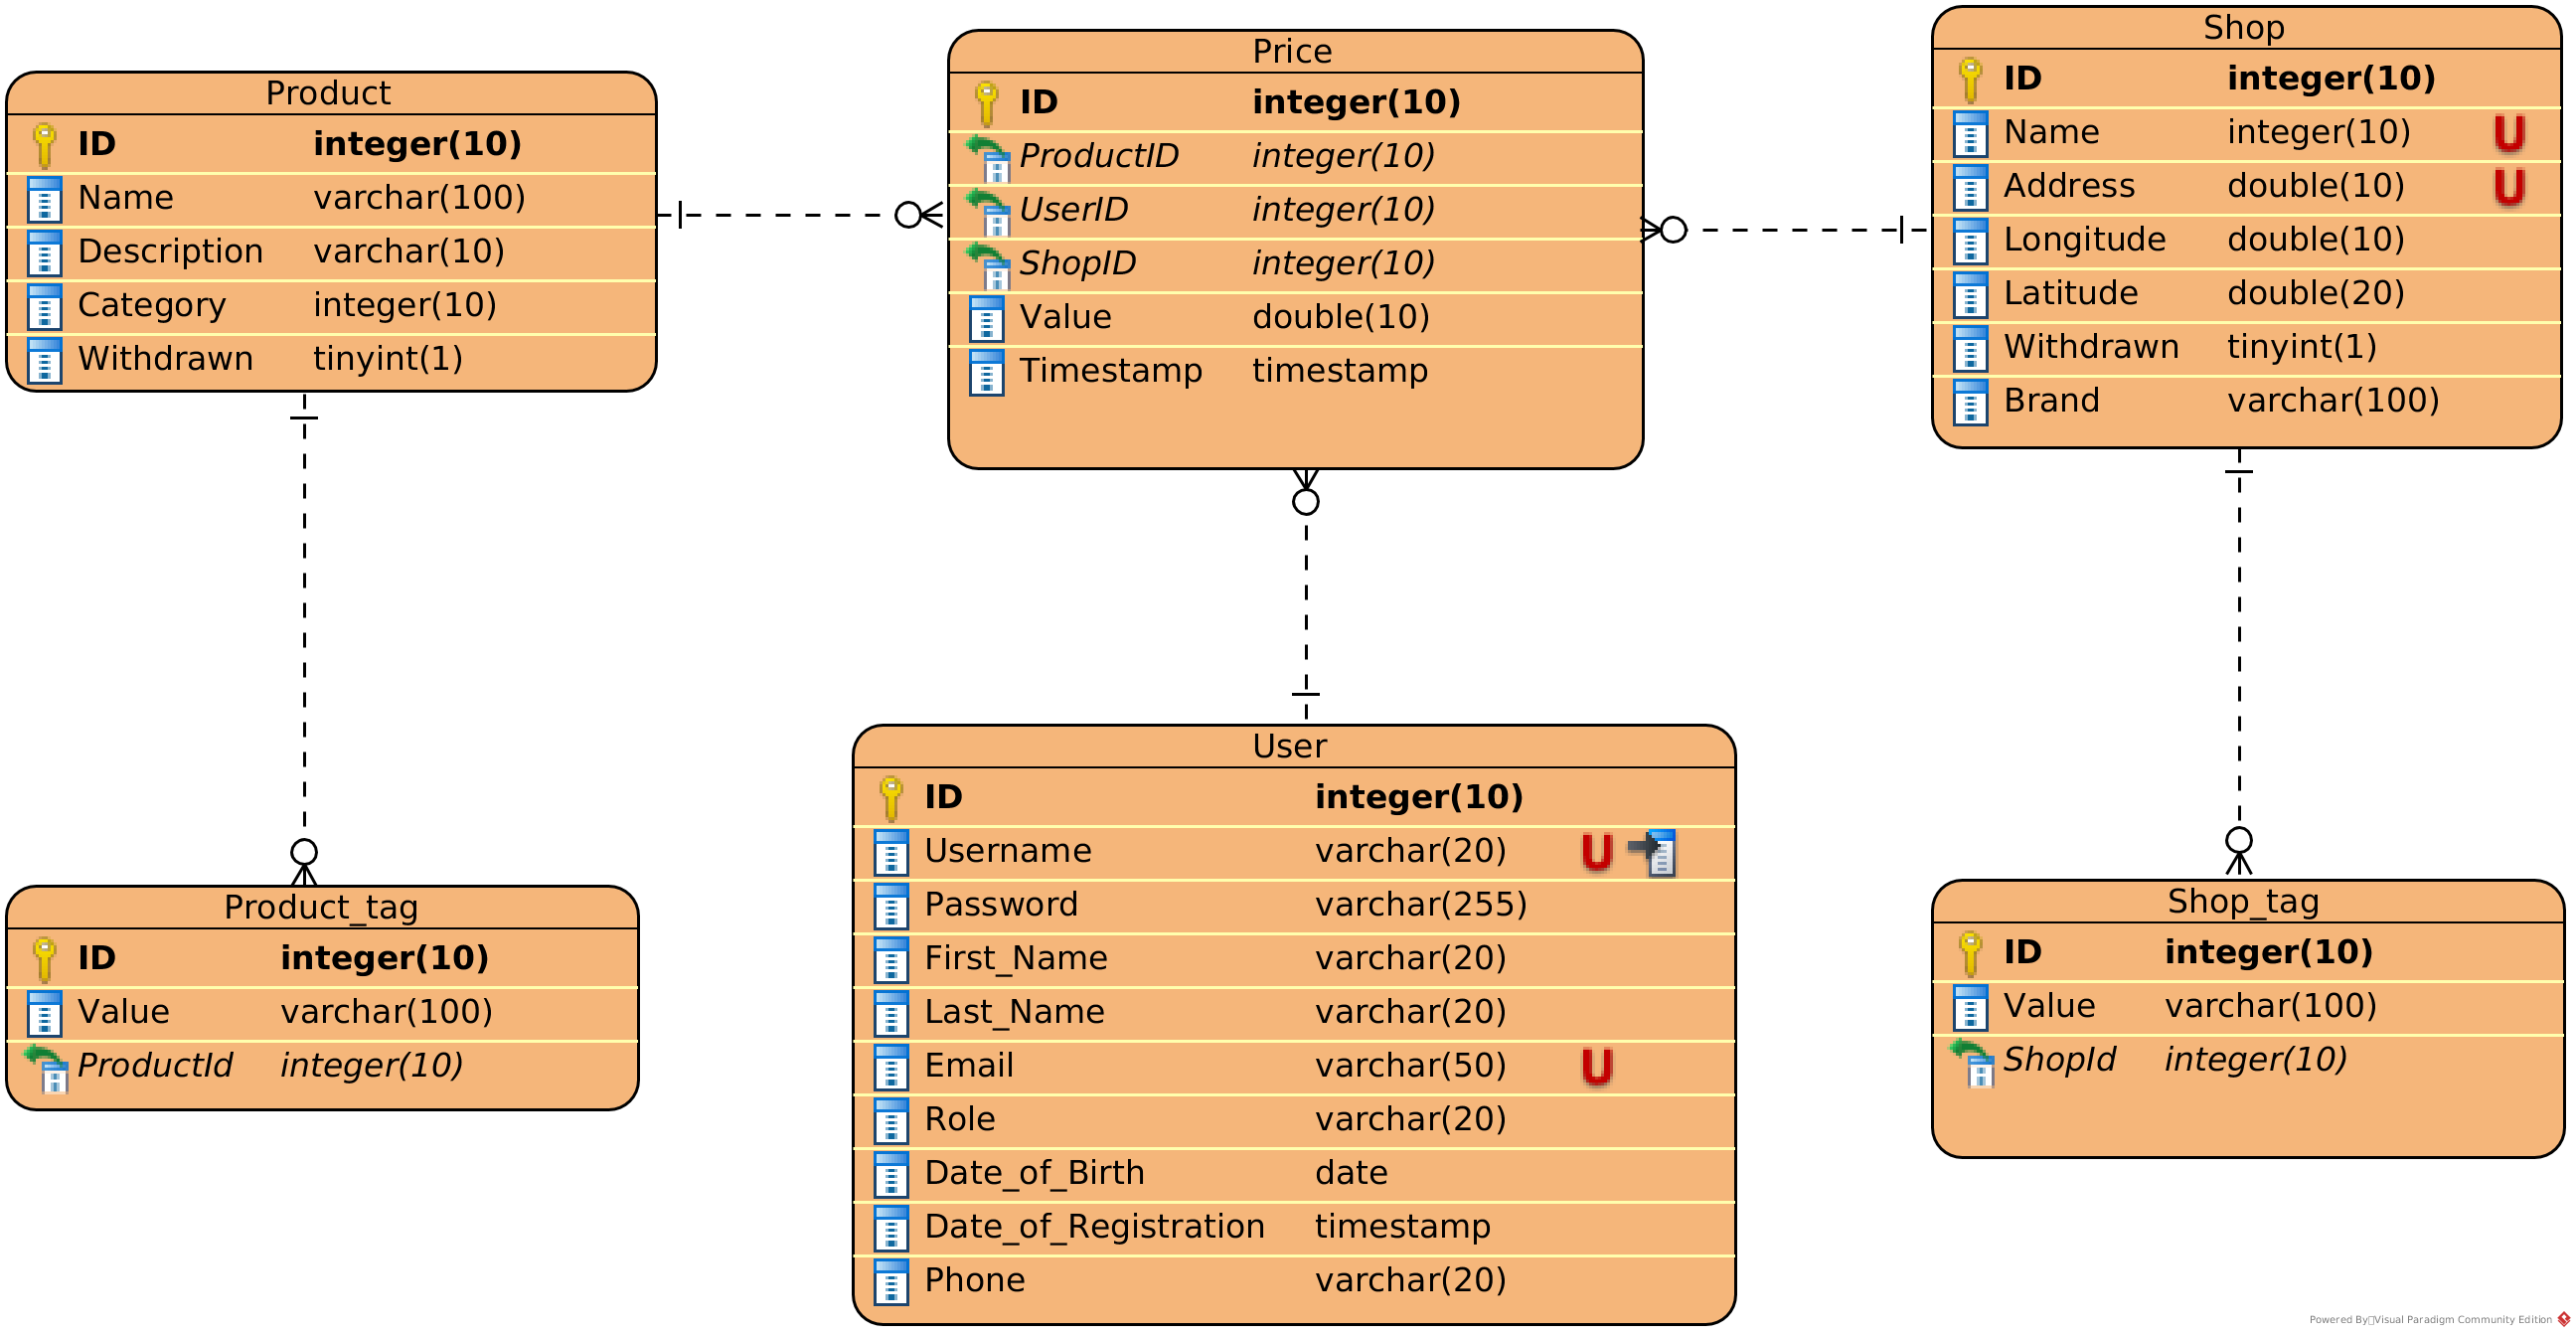
\includegraphics[width = \linewidth]{media/DB/ER.png}
    \caption{Entity-Relationship Diagram (ERD)}
\end{figure}

\begin{figure}[H]
    \centering
    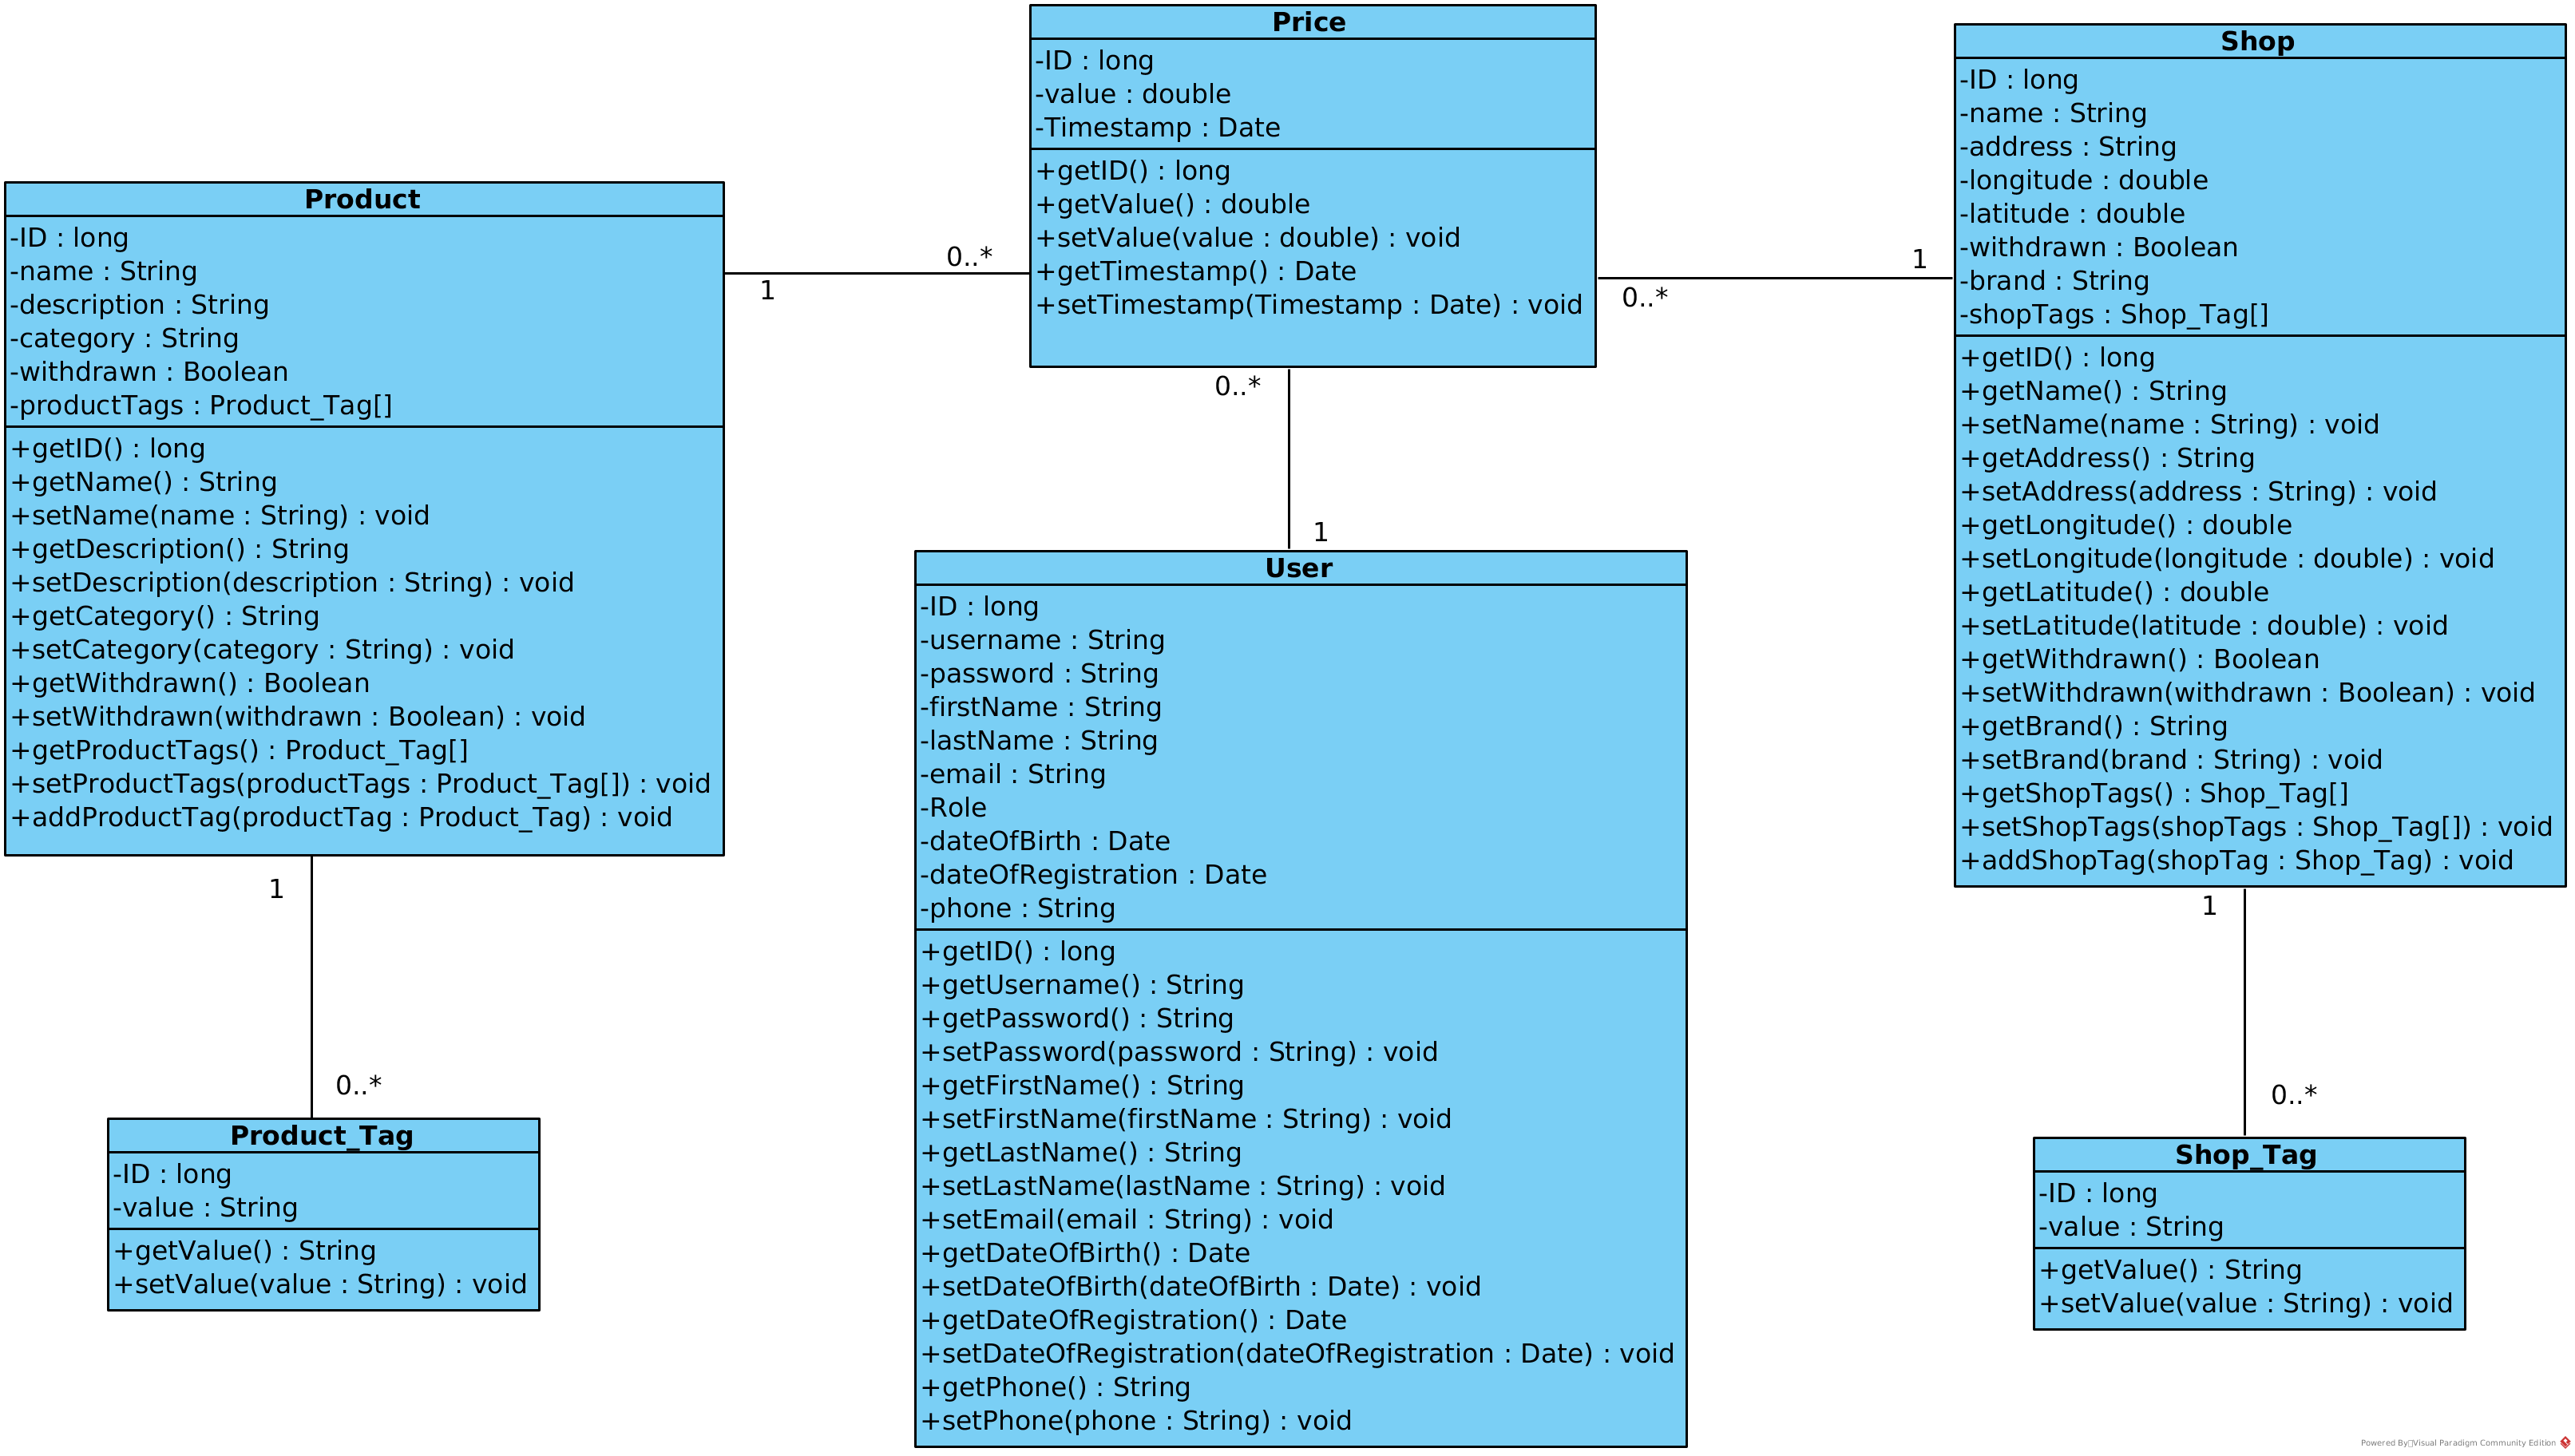
\includegraphics[width = \linewidth]{media/DB/Database.png}
    \caption{Class Diagram}
\end{figure}




% https://en.wikipedia.org/wiki/Data_integrity
\subsubsection{Προδιαγραφές ακεραιότητας δεδομένων}
Παρακάτω παρουσιάζονται οι κανόνες ακεραιότητας και εγκυρότητας δεδομένων τοσο σε φυσικό όσο και σε λογικό επίπεδο.

\paragraph*{Φυσικό Επίπεδο}
\begin{enumerate}
    \item Χρήση συστοιχιών RAID για αποφυγή σφαλμάτων υλικού στη βάση δεδομένων.
    \item Χρήση error detecting algorithms ή αλλιώς error-correcting codes (π.χ. parity bit)
\end{enumerate}

\paragraph*{Λογικό Επίπεδο}
\begin{enumerate}
    \item Αρχές Μεθοδολογίας ACID: Η βάση δεομένων μας θα πρέπει να ακολουθει κανόνες ACID για τις δοσοληψίες της.
    \item Entity Integrity: Ύπαρξη μοναδικών primary keys για κάθε οντότητα.
    \item Referential integrity: Ύπαρξη foreign keys μεταξύ οντοτήτων.
    \item Domain integrity: Κάθε πεδίο πρέπει να έχει ένα συγκεκριμένο τύπο δεδομένων.
    \item User-defined integrity: Χρήση user defined rules (π.χ. NOT NULL κ.τ.λ)
\end{enumerate}

\subsubsection{Προδιαγραφές διατήρησης δεδομένων}
Παρακάτω παρουσιάζονται προδιαγραφές διατήρησης δεδομένων
% https://www.mssqltips.com/sqlservertutorial/2210/maintenance-tasks-for-sql-server/
\begin{itemize}
    \item Δημιουργία αντιγράφων backup της βάσης δεδομένων και των log files της.
    \item Ανανέωση στατιστικών στοιχείων στη βάση δεδομένων για optimized λειτουργία.
    \item Τακτικοί έλεγχοι για τη συνέπεια της βάσης δεδομένων.
    \item Τακτικό rebuild των indices της βάσης δεδομένων
    \item Τακτικά clean up tasks
    \item Shrinking δεδομένων και αφαίρεση άδειων σελίδων από τη βάση δεδομένων.
    \item Συνεχή updates για τη χρήση των πλέον πρόσφατων εκδόσεων λογισμικού.

\end{itemize}
